%--------------------------------------------------
\subsection{Prototipo 4: Integración de pantalla para ejecutar algoritmo k-means}
Dentro de este prototipo se satisface el requerimiento funcional \hyperlink{RFPA}{Ejecutar algoritmo de agrupamiento}, definido previamente en el capítulo del ``Bosquejo general de la aplicación''  con el título de ``Requerimientos funcionales del Panel de Administración''. \\ \par

\FloatBarrier

%--------------------------------------------------
\subsubsection{Análisis}

\title{\textbf{Diagrama de casos de uso \\}}
En la figura \ref{casosusomiddleware2} se puede visualizar el diagrama de casos de uso actualizado.
\\
Modificaciones realizadas: 
\begin{itemize}
\item Ninguna.
\end{itemize}

\FloatBarrier
\begin{figure}[htbp!]
		\centering
			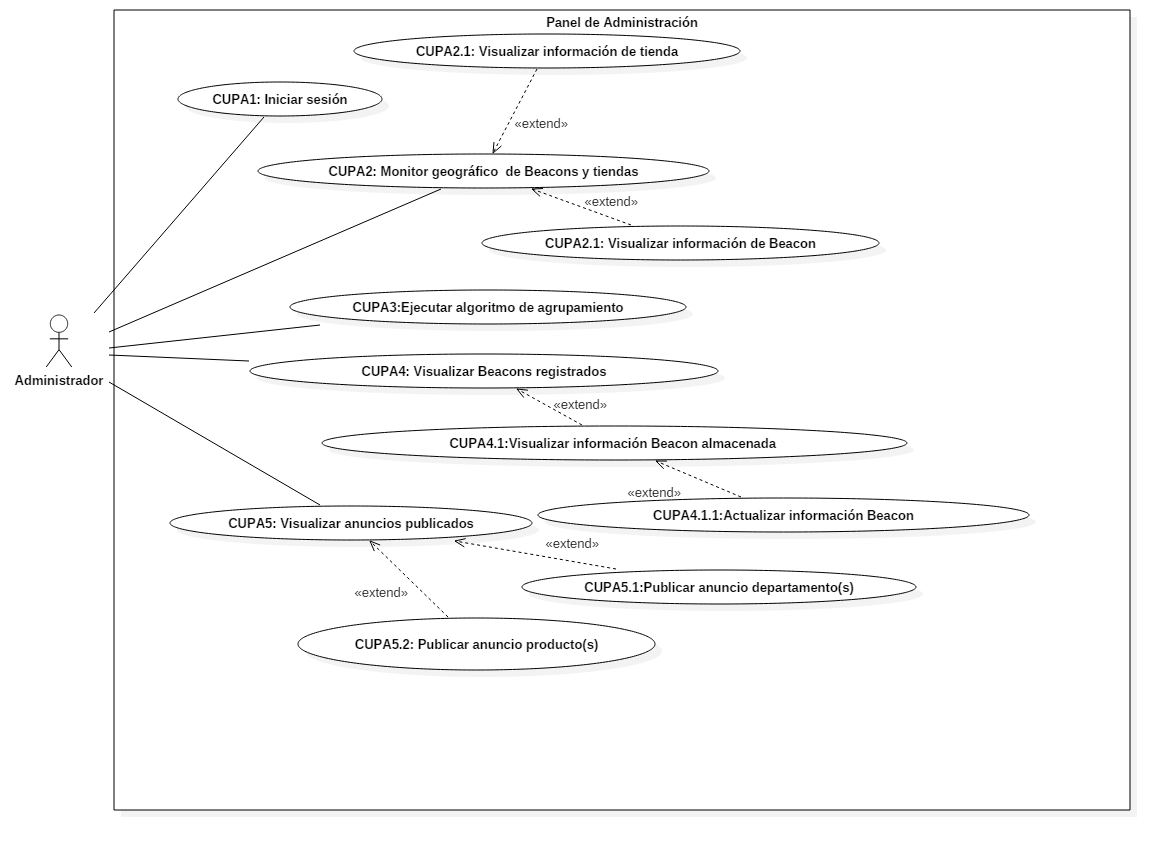
\includegraphics[width=1.1 \textwidth]{imagenes/CU/middleware}
		\caption{Casos de uso PA.}
		\label{casosdeusoPA}
\end{figure}
\FloatBarrier

%--------------------------------------------------
\subsubsection{Diseño}

\title{\textbf{Diagramas de secuencia \\}}
Las figuras \ref{PADS:ejecutarcluster} muestra el diagrama satisface el caso de uso \hyperlink{casosdeusoPA}{Ejecutar algoritmo de agrupamiento} que se muestra en el diagrama de casos de uso. \\ \textit{El diagrama fue separado en tres figuras para mejor visualización (\ref{PADS:ejecutarcluster}, \ref{PADS:ejecutarcluster1}, \ref{PADS:ejecutarcluster2})}
\FloatBarrier
\begin{figure}[htbp!]
		\centering
			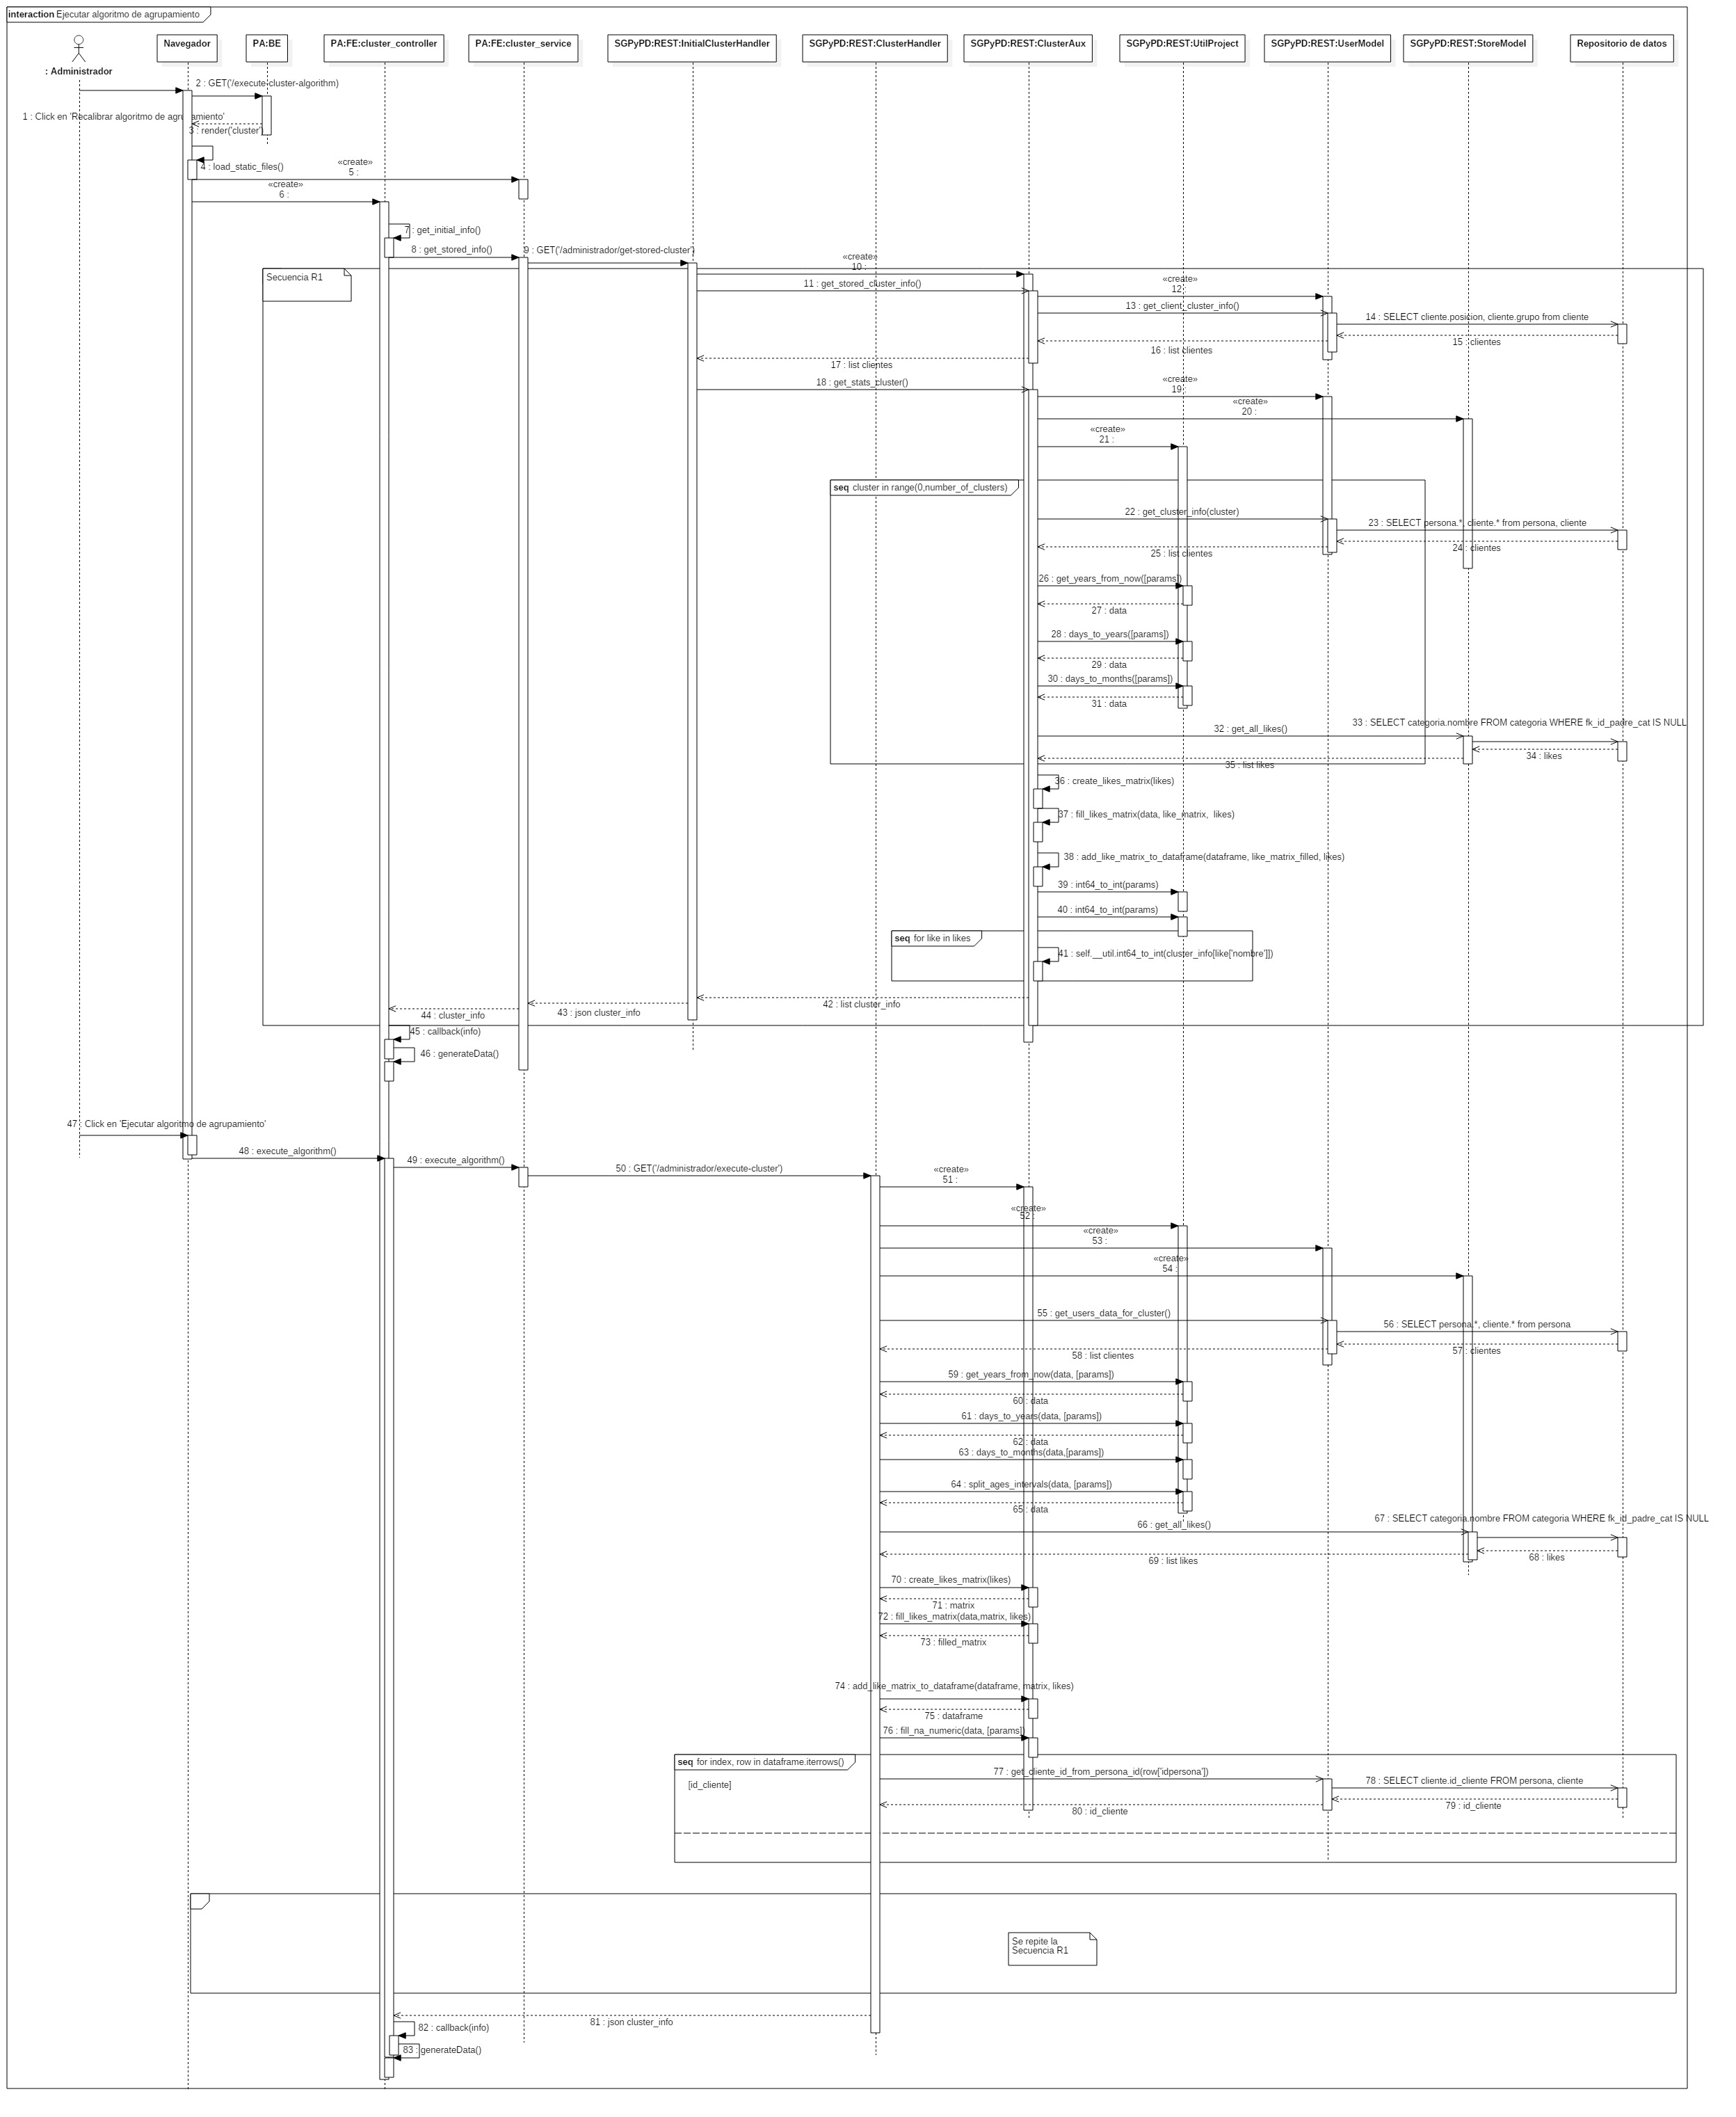
\includegraphics[width=1 \textwidth]{imagenes/DSRuben/CLUSTER}
		\caption{Diagrama de secuencia Ejecutar algoritmo de agrupamiento (Visualización completa).}
		\label{PADS:ejecutarcluster}
\end{figure}
\FloatBarrier

\FloatBarrier
\begin{figure}[htbp!]
		\centering
			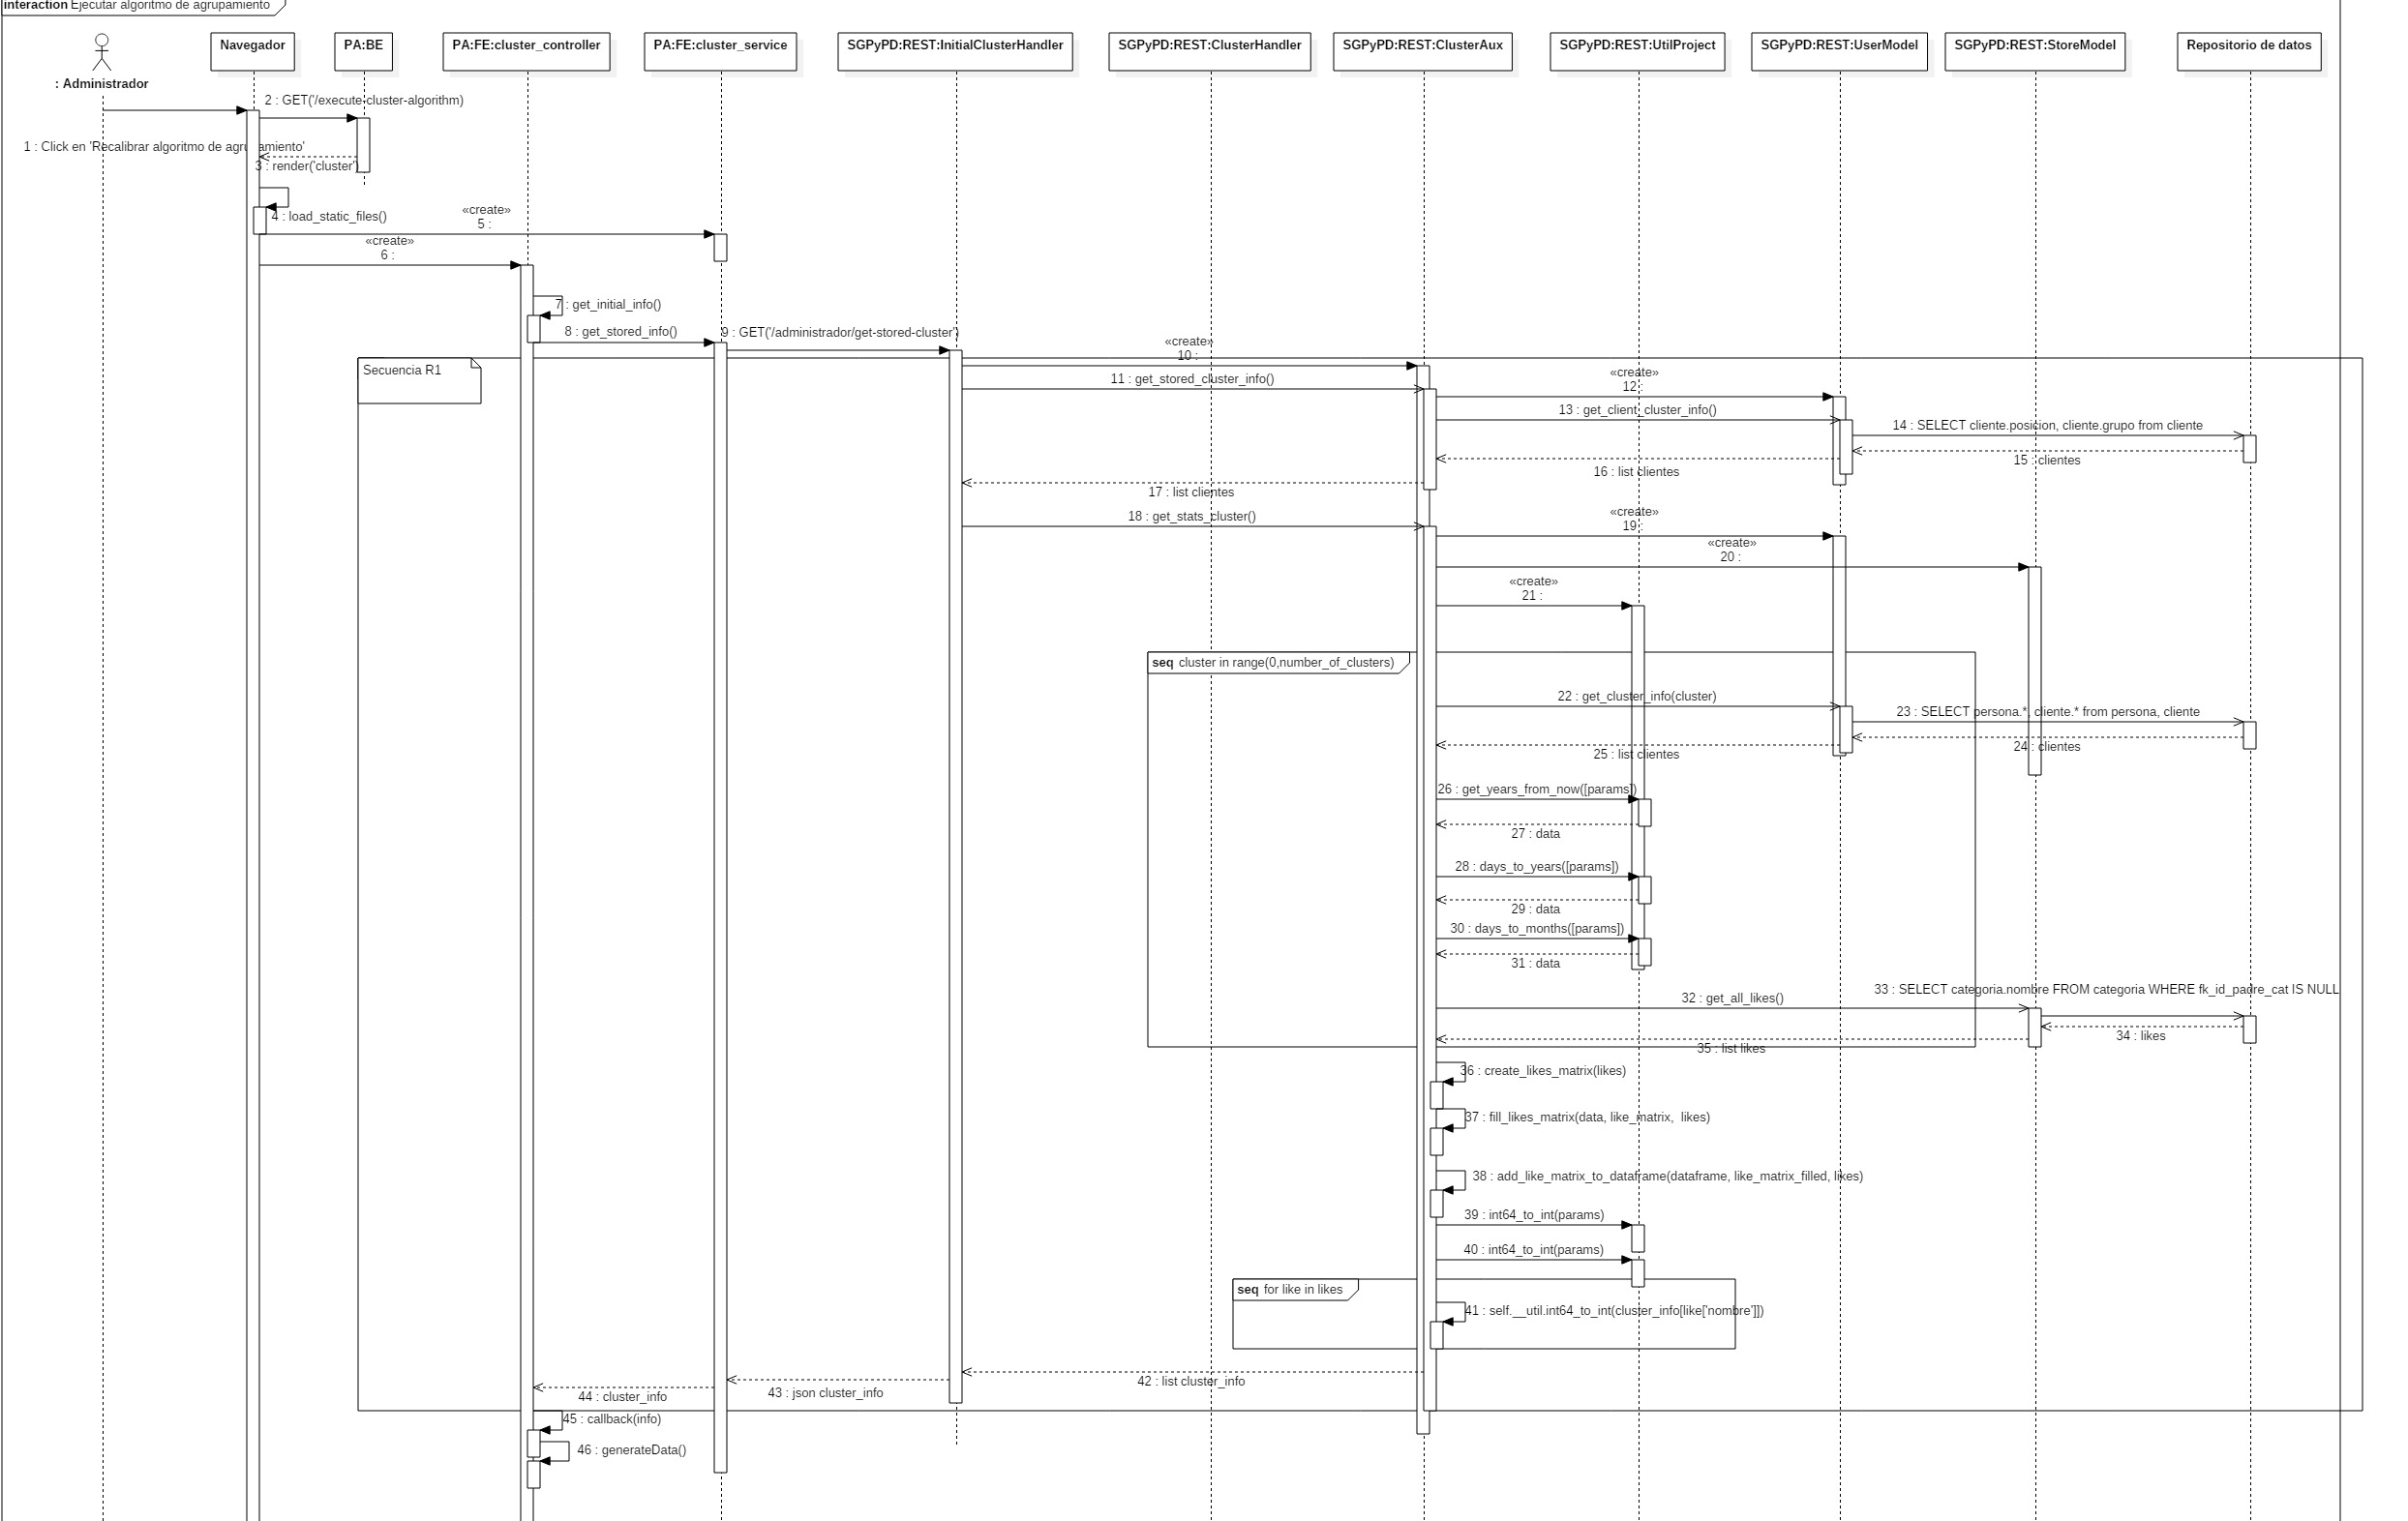
\includegraphics[width=1.1 \textwidth]{imagenes/DSRuben/CLUSTER1}
		\caption{Diagrama de secuencia Ejecutar algoritmo de agrupamiento (Parte 1). }
		\label{PADS:ejecutarcluster1}
\end{figure}
\FloatBarrier

\FloatBarrier
\begin{figure}[htbp!]
		\centering
			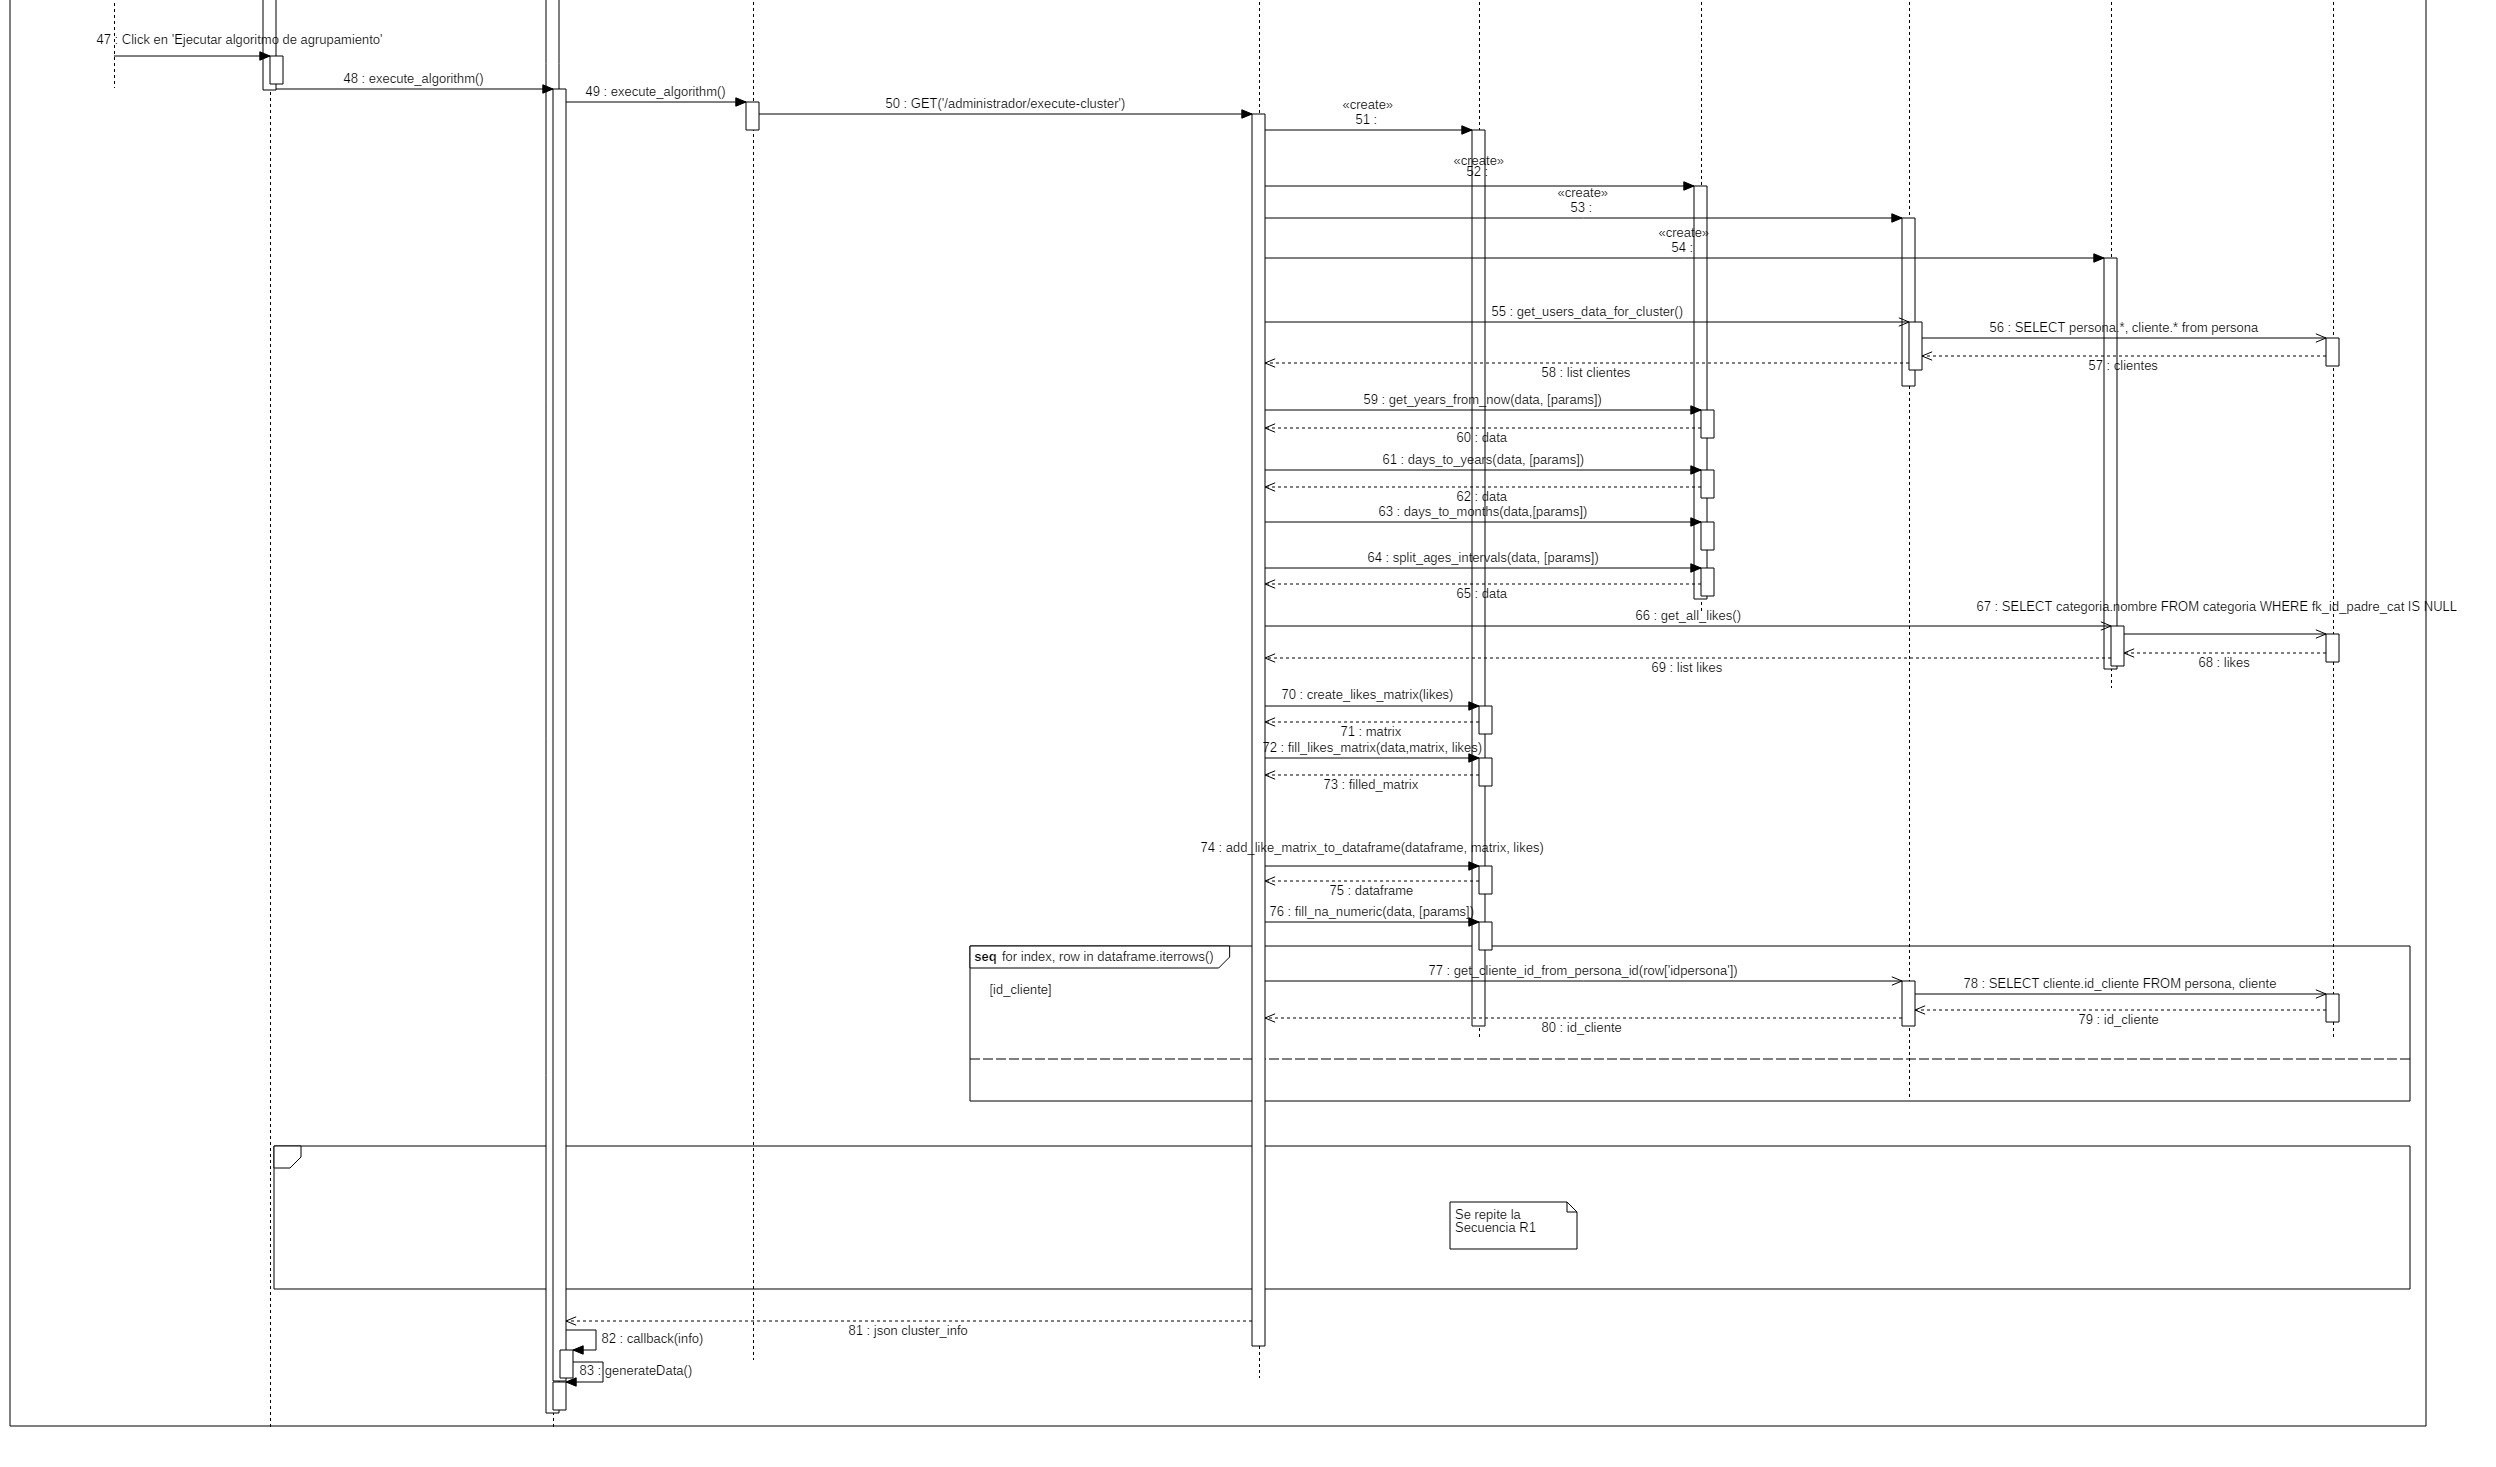
\includegraphics[width=1.1 \textwidth]{imagenes/DSRuben/CLUSTER2}
		\caption{Diagrama de secuencia Ejecutar algoritmo de agrupamiento (Parte 2). }
		\label{PADS:ejecutarcluster2}
\end{figure}
\FloatBarrier

\title{\textbf{Diseño de interfaz de usuario \\}}

En las Figuras \ref{PA:cluster1} y \ref{PA:cluster2} se muestra la interfaz de usuario que satisface el requerimiento \hyperlink{RFPA}{Ejecutar algoritmo de agrupamiento}.
\FloatBarrier
\begin{figure}[htbp!]
		\centering
			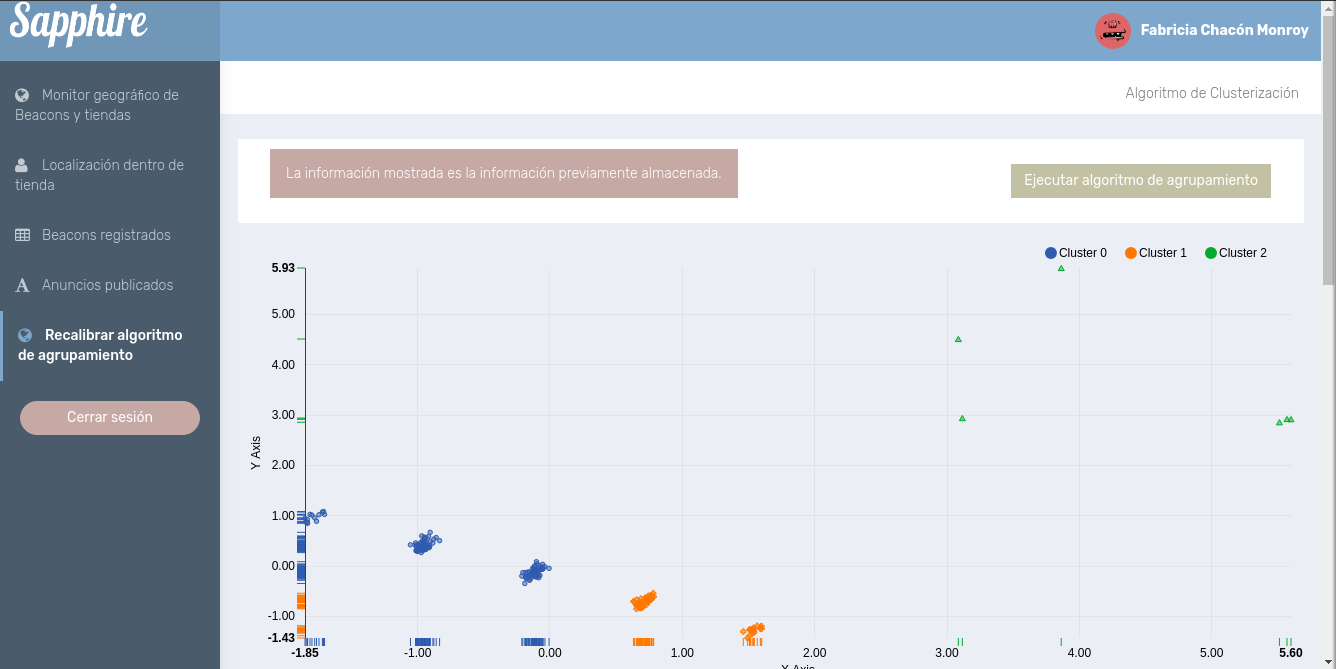
\includegraphics[width=1 \textwidth]{imagenes/UI/prototipo4/cluster}
		\caption{UIPanel37: Ejecutar algoritmo de agrupamiento (Parte 1).}
		\label{PA:cluster1}
\end{figure}
\FloatBarrier

\FloatBarrier
\begin{figure}[htbp!]
		\centering
			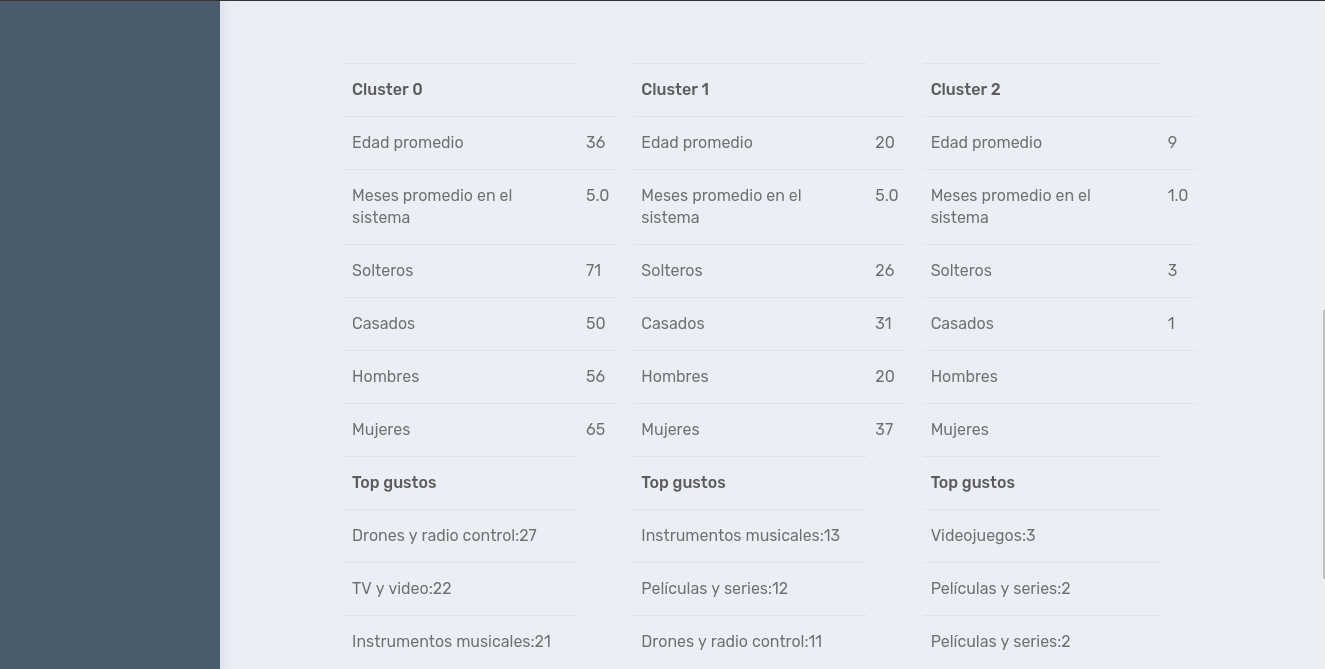
\includegraphics[width=1 \textwidth]{imagenes/UI/prototipo4/cluster2}
		\caption{UIPanel38: Ejecutar algoritmo de agrupamiento (Parte 2).}
		\label{PA:cluster2}
\end{figure}
\FloatBarrier


\paragraph{Flujo de navegación del Panel de Administración.} ~\\

La figura \ref{PA:flujo4} muestra como es el flujo de navegación general del Panel de Admnistración.

\FloatBarrier
\begin{figure}[htbp!]
		\centering
			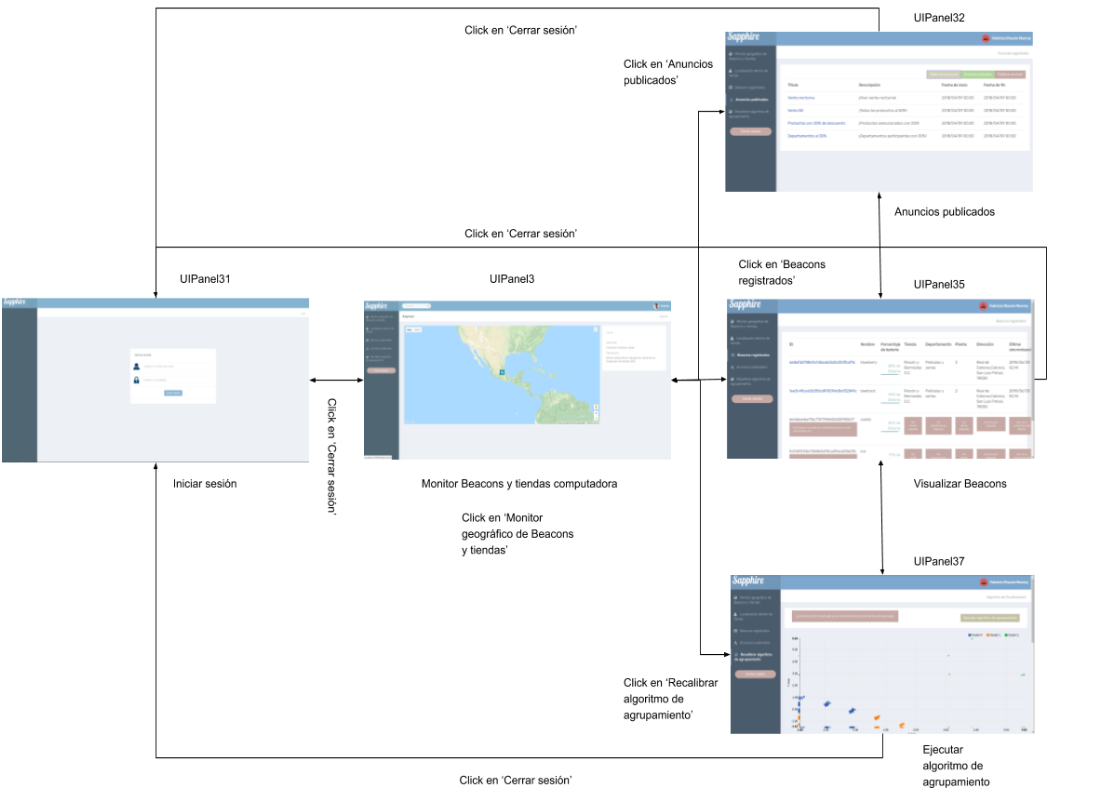
\includegraphics[width=1 \textwidth]{imagenes/paneladminmapa/general4}
		\caption{Flujo de navegación general Panel de Administración.}
		\label{PA:flujo4}
\end{figure}
\FloatBarrier



La figura \ref{PA:flujoBeacons} muestra como es el flujo de navegación de la pantalla \textbf{Beacons registrados}.

\FloatBarrier
\begin{figure}[htbp!]
		\centering
			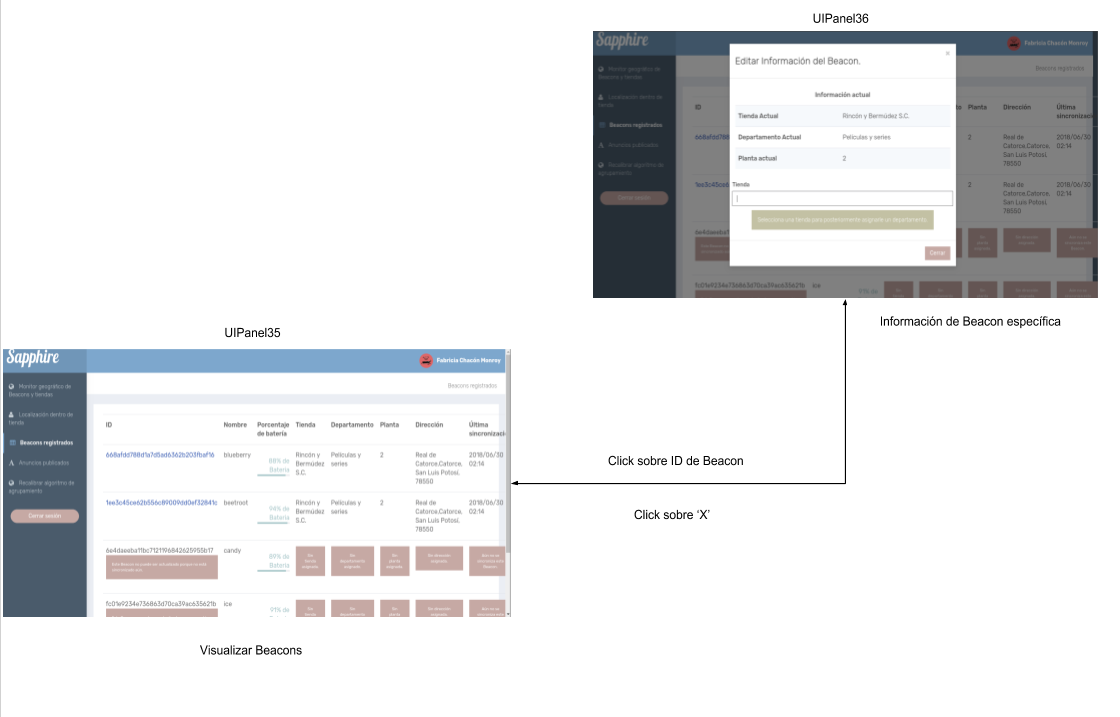
\includegraphics[width=1 \textwidth]{imagenes/paneladminmapa/beacons3}
		\caption{Flujo de navegación de pantalla Beacons registrados.}
		\label{PA:flujoBeacons}
\end{figure}
\FloatBarrier

La figura \ref{PA:flujoBeacons} muestra como es el flujo de navegación de la pantalla \textbf{Anuncios publicados}.

\FloatBarrier
\begin{figure}[htbp!]
		\centering
			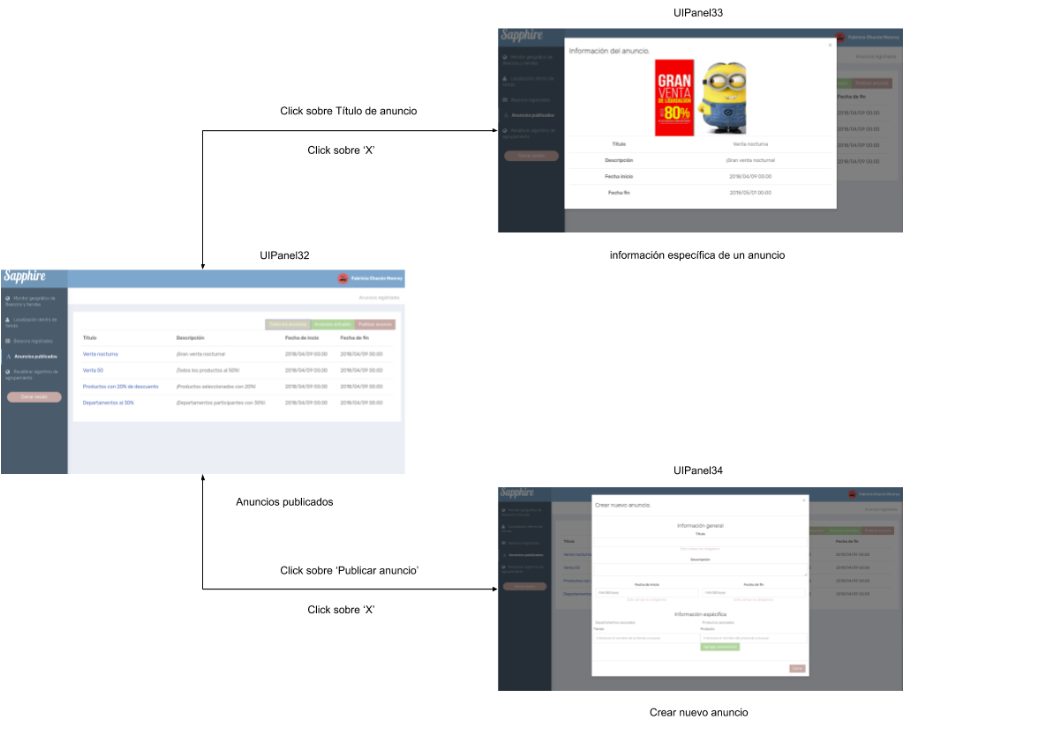
\includegraphics[width=1 \textwidth]{imagenes/paneladminmapa/anuncios3}
		\caption{Flujo de navegación de pantalla Anuncios publicados.}
		\label{PA:flujoAnuncios}
\end{figure}
\FloatBarrier

\subsubsection{Pruebas}

\textit{Las pruebas del sistema fueron hechas sobre una laptop Lenovo Thinkpad T460 con las siguientes carácteristicas:\\}
\begin{itemize}
\item Procesador Intel® Core™ i5-5300U (3M Cache, hasta 2,90 GHz).
\item 8 GB RAM.
\item 240 GB Solid State Drive ROM.
\item Sistema Operativo Fedora 27.
\end{itemize}
%%%%%%%%%%%%%%%%%%%%% PRUEBA 1
\title{\textbf{Prueba 1.}}

\begin{itemize}
\item Número de clientes:184
\item Número de clusters: 2
\end{itemize}

\FloatBarrier
\begin{figure}[htbp!]
		\centering
			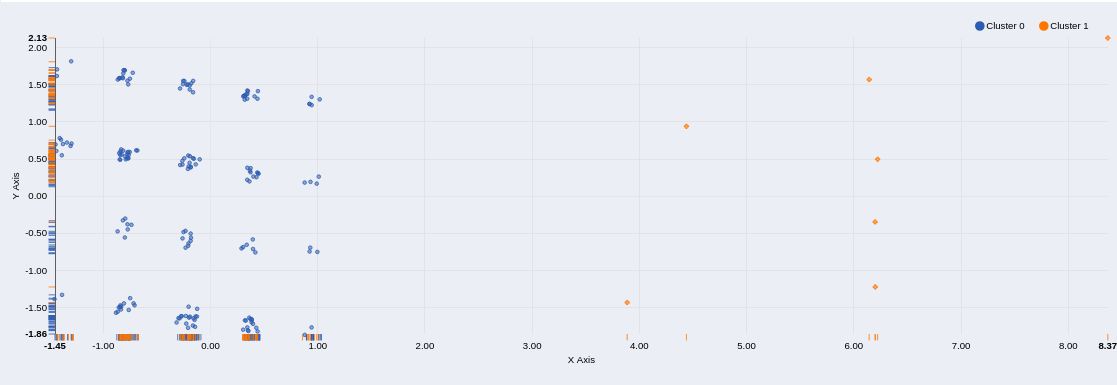
\includegraphics[width=1 \textwidth]{imagenes/pruebassistemarecom/cluster2_1}
		\caption{Prueba 1.}
\end{figure}
\FloatBarrier

\FloatBarrier
\begin{figure}[htbp!]
		\centering
			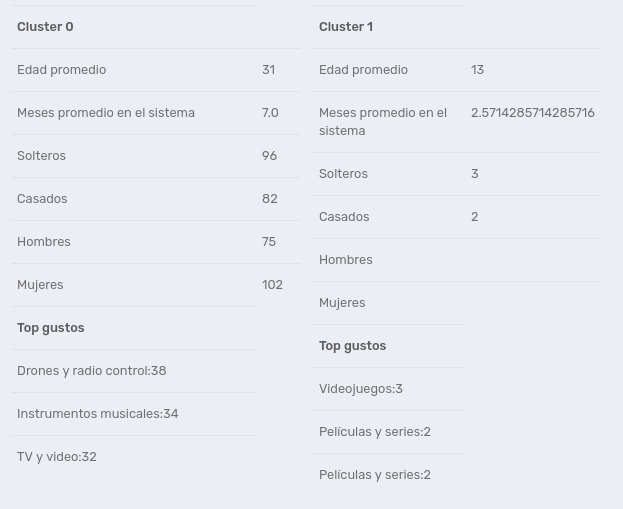
\includegraphics[width=1 \textwidth]{imagenes/pruebassistemarecom/cluster2_2}
		\caption{Prueba 1 características de cada cluster.}
\end{figure}
\FloatBarrier

%%%%%%%%%%%%%%%%%%%%%%%%%%% prueba 2

\title{\textbf{Prueba 2.}}

\begin{itemize}
\item Número de clientes:184
\item Número de clusters: 3
\end{itemize}

\FloatBarrier
\begin{figure}[htbp!]
		\centering
			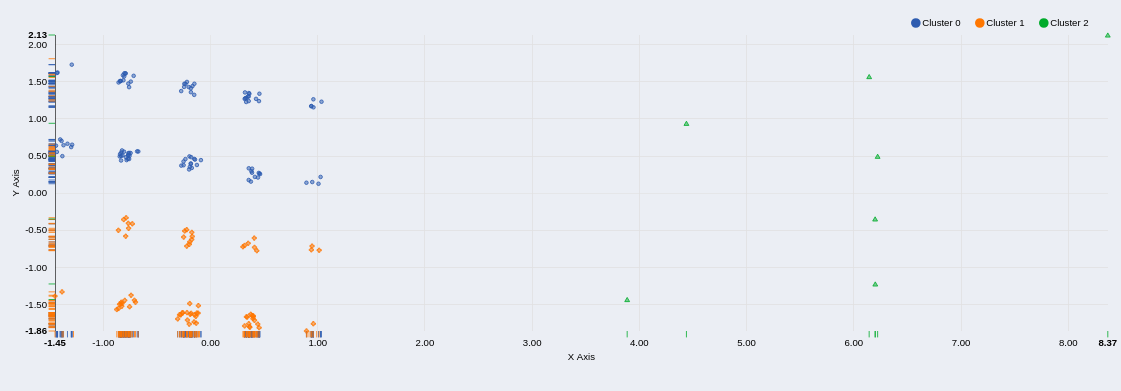
\includegraphics[width=1 \textwidth]{imagenes/pruebassistemarecom/cluster3_1}
		\caption{Prueba 2.}
		\label{PA:pruebafinal}
\end{figure}
\FloatBarrier

\FloatBarrier
\begin{figure}[htbp!]
		\centering
			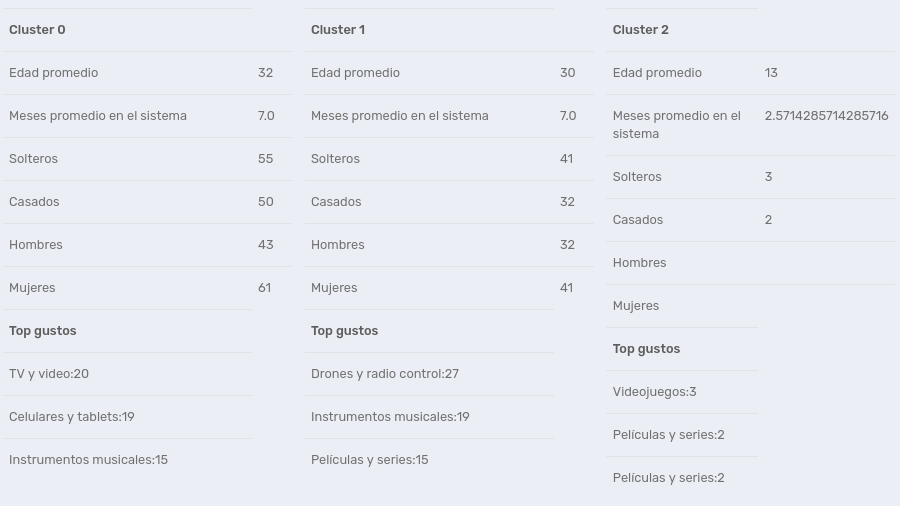
\includegraphics[width=1 \textwidth]{imagenes/pruebassistemarecom/cluster3_2}
		\caption{Prueba 2 características de cada cluster.}
\end{figure}
\FloatBarrier


%%%%%%%%%%%%%%%%%%%%%%%%%%% prueba 3

\title{\textbf{Prueba 3.}}

\begin{itemize}
\item Número de clientes:184
\item Número de clusters: 4
\end{itemize}

\FloatBarrier
\begin{figure}[htbp!]
		\centering
			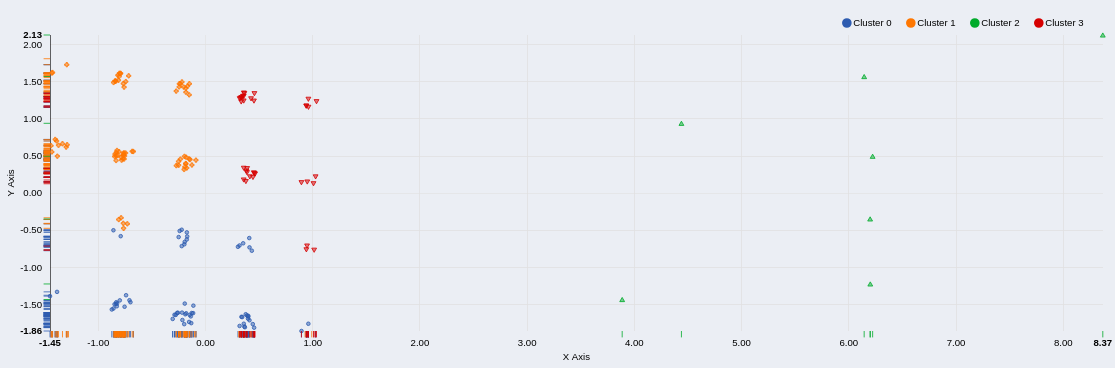
\includegraphics[width=1 \textwidth]{imagenes/pruebassistemarecom/cluster4_1}
		\caption{Prueba 3.}
\end{figure}
\FloatBarrier

\FloatBarrier
\begin{figure}[htbp!]
		\centering
			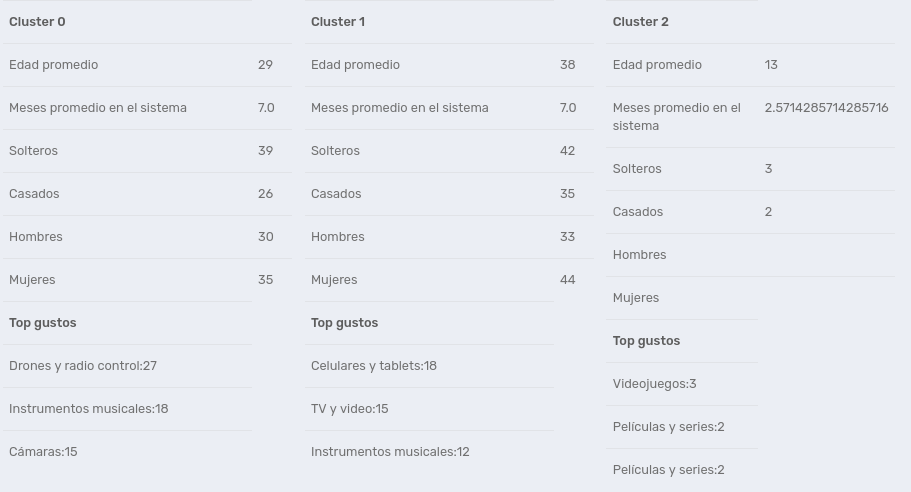
\includegraphics[width=1 \textwidth]{imagenes/pruebassistemarecom/cluster4_2}
		\caption{Prueba 3 características de cada cluster (Parte 1).}
\end{figure}
\FloatBarrier

\FloatBarrier
\begin{figure}[htbp!]
		\centering
			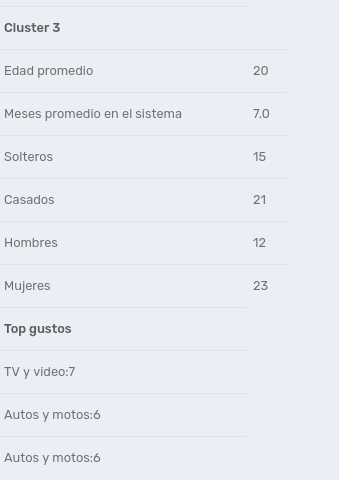
\includegraphics[width=0.4 \textwidth]{imagenes/pruebassistemarecom/cluster4_3}
		\caption{Prueba 3 características de cada cluster (Parte 2).}
\end{figure}
\FloatBarrier



\subsubsection{Conclusiones}
De acuerdo con las pruebas realizadas se decidió que el número de clusters óptimo es tres, ya que, separa los datos de una manera muy natural (como se muestra en la gráfica \ref{PA:pruebafinal}) y a pesar de que existe una muy poca diferencia en la edad promedio entre el cluster 0 y el cluster los gustos de cada cluster son diferentes y eso es un factor importante a tomar en cuenta.